\noindent
\begin{minipage}[t]{0.26\textwidth}
    \vspace*{31mm}
    {\footnotesize\raggedright
    Hình 2 biểu diễn đồ thị của hàm số $f$ trong Ví dụ 1 và đạo hàm $f'$ của nó. Lưu ý rằng $f'(x)$ mang giá trị dương khi $f$ đồng biến và mang giá trị âm khi $f$ nghịch biến.\par}
    
    \vspace{3mm}
    \centering
    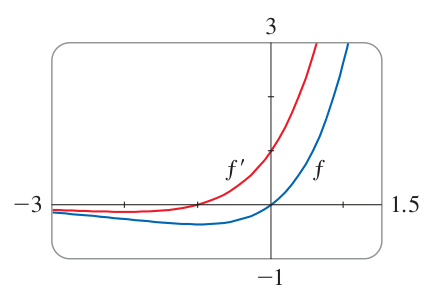
\includegraphics[width=\linewidth]{images/p0221_fig1.png}
    
    \vspace{2mm}
    \raggedright
    \textbf{\textsf{\footnotesize HÌNH 2}}\par

    \vspace{48mm}
    {\footnotesize\raggedright
    Trong Ví dụ 2, $a$ và $b$ là các hằng số. Trong toán học, theo thông lệ ta dùng các chữ cái ở đầu bảng chữ cái để biểu thị hằng số và các chữ cái ở cuối bảng chữ cái để biểu thị biến số.\par}
\end{minipage}%
\hfill
\begin{minipage}[t]{0.70\textwidth}
    \raggedright
    Nói bằng lời, Quy tắc nhân phát biểu rằng \emph{đạo hàm của tích hai hàm số bằng hàm thứ nhất nhân với đạo hàm của hàm thứ hai cộng với hàm thứ hai nhân với đạo hàm của hàm thứ nhất}.

    \vspace{3.5mm}
    \textbf{\textsf{\color{stewartcyan}VÍ DỤ 1}}\quad \textbf{(a)}\enspace Nếu $f(x) = xe^x$, hãy tìm $f'(x)$.\par
    \vspace{1mm}
    \textbf{(b)}\enspace Tìm đạo hàm cấp $n$, $f^{(n)}(x)$.

    \vspace{3mm}
    \textbf{\textsf{\color{stewartcyan}LỜI GIẢI}}\quad \textbf{(a)}\enspace Theo Quy tắc nhân, ta có
    \begin{align*}
    f'(x) &= \frac{d}{dx}(xe^x) \\[1mm]
          &= x\frac{d}{dx}(e^x) + e^x\frac{d}{dx}(x) \\[1mm]
          &= xe^x + e^x \cdot 1 = (x + 1)e^x
    \end{align*}

    \textbf{(b)}\enspace Áp dụng Quy tắc nhân lần thứ hai, ta được
    \begin{align*}
    f''(x) &= \frac{d}{dx}\bigl[(x + 1)e^x\bigr] \\[1mm]
           &= (x + 1)\frac{d}{dx}(e^x) + e^x\frac{d}{dx}(x + 1) \\[1mm]
           &= (x + 1)e^x + e^x \cdot 1 = (x + 2)e^x
    \end{align*}
    Tiếp tục áp dụng Quy tắc nhân, ta được
    \[
    f'''(x) = (x + 3)e^x \qquad f^{(4)}(x) = (x + 4)e^x
    \]
    Trên thực tế, mỗi lần lấy đạo hàm liên tiếp đều cộng thêm một số hạng $e^x$, do đó
    \[
    f^{(n)}(x) = (x + n)e^x \tag*{\color{stewartcyan}\blacksquare}
    \]

    \vspace{2.5mm}
    \textbf{\textsf{\color{stewartcyan}VÍ DỤ 2}}\quad Tính đạo hàm của hàm số $f(t) = \sqrt{t}\,(a + bt)$.

    \vspace{2mm}
    \textbf{\textsf{\color{stewartcyan}LỜI GIẢI 1}}\quad Áp dụng Quy tắc nhân, ta có
    \begin{align*}
    f'(t) &= \sqrt{t}\,\frac{d}{dt}(a + bt) + (a + bt)\frac{d}{dt}(\sqrt{t}) \\[1.5mm]
          &= \sqrt{t}\cdot b + (a + bt)\cdot \frac{1}{2}t^{-1/2} \\[1.5mm]
          &= b\sqrt{t} + \frac{a + bt}{2\sqrt{t}} = \frac{a + 3bt}{2\sqrt{t}}
    \end{align*}

    \vspace{1mm}
    \textbf{\textsf{\color{stewartcyan}LỜI GIẢI 2}}\quad Nếu trước hết ta sử dụng các quy tắc về lũy thừa để viết lại $f(t)$, thì ta có thể tính đạo hàm trực tiếp mà không cần dùng Quy tắc nhân.
    \begin{align*}
    f(t) &= a\sqrt{t} + bt\sqrt{t} = at^{1/2} + bt^{3/2} \\[1.5mm]
    f'(t) &= \frac{1}{2}at^{-1/2} + \frac{3}{2}bt^{1/2}
    \end{align*}
    kết quả này tương đương với đáp số tìm được trong Lời giải 1.\hfill{\color{stewartcyan}\blacksquare}
\end{minipage}
